\section{Motivation}
%
We will start the introduction by giving a motivation to the work done in this thesis, and try to put it in a larger context.
The ultimate goal is to provide clean energy%
\footnote{Words like "energy consumption" will here be referring to conversion of energy in a low entropy state to the same amount of energy in a higher entropy state.
}
%
to a growing population with a elevated standard of living compared to just $100$ years ago.
One projection of the increased energy demand is given in \cref{fig:energyDemand}.
%
\begin{figure}[htb]
    \begin{center}
        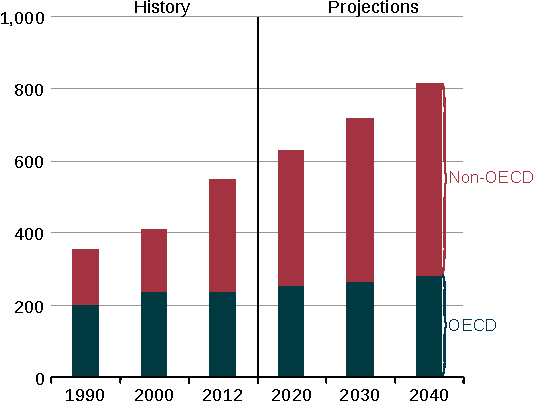
\includegraphics{fig/intro/energyDemand}
    \end{center}
    \caption{Historic and projected energy consumption from \cite{UEIA2016book}.
    The ordinate is given in quadrillion British thermal unit, which approximately equals $10^{18} \J$.
    }
    \label{fig:energyDemand}
\end{figure}

\noindent
As the bulkpart of the current energy consumption is provided by limited energy sources, a more sustainable approach is needed.

One candidate for a more sustainable energy production is through thermonuclear fusion.
We will here give a short summary of the process.
For more introduction on the topic, see \cite{Freidberg2008book}.
If two nuclei can overcome the electrostatic Coulomb-barrier (with the "help" of quantum tunneling), they can fuse into a heavier nuclues.
The process will release a surplus of energy if the mass of the resulting nuclues is lighter than the sum of the two initial nuclei.
The main reaction sougth is the $\text{D}-\text{T}$ reaction, which can be summarized as
%
\begin{align*}
    \text{D} + \text{T} \to \text{He}^4 + \text{n} + 17.6 \text{MeV},
\end{align*}
%
where the deuterium $\text{D}$ can be destilled from sea water, whereas the tritium $\text{T}$ must be produce due to scarce aviability and a short half-life of $12.3$ years.
Probably the easiest way to obtain $\text{T}$ is by breeding it from lithium through the process
%
\begin{align*}
    \text{Li}^6 + \text{n} &\to \text{T} + \text{He}^4 + 4.8 \text{MeV}\\
    \text{Li}^7 + \text{n} &\to \text{T} + \text{He}^4 + \text{n} - 2.5 \text{MeV}.
\end{align*}
%
The need of $\text{Li}$ could theoretically be replaced by tritium breeding from the $\text{D}-\text{D}$ reaction
%
\begin{align*}
    \text{D} + \text{D} \to \text{T} + \text{p} + 4.03 \text{MeV}.
\end{align*}
%

However, this is a much harder reaction to achieve, as it requires subtatinally higher temperatures.
The potential benefits and sustainability of fusion energy is given in \cref{fig:potFusion}.
%
\begin{figure}[htbp]
    \centering
    \begin{subfigure}[h]{1.00\textwidth}
        \centering
        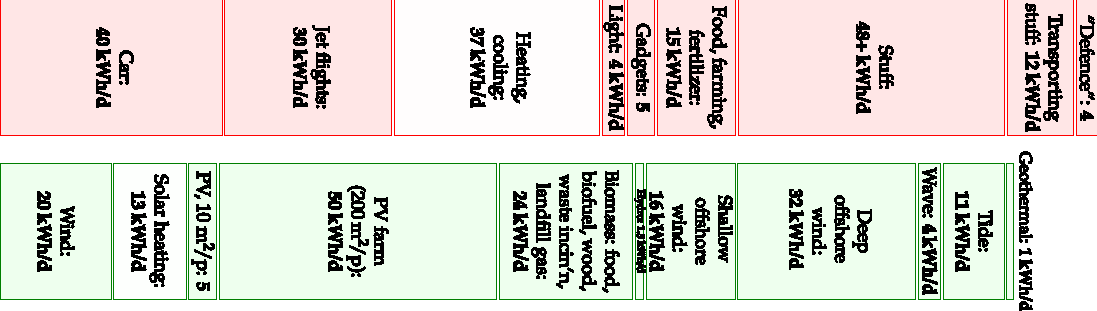
\includegraphics[width=1.0\textwidth]{fig/intro/energyConsumption}
        \caption{A "back-of-the-envelope-calculation" of the average energy consumption in the UK ,$125 \text{kWh/day/person}$, (top) together with an idealized potential for renewable energy in the UK (bottom).}
    \label{fig:energyConsumption}
    \end{subfigure}%
    \vfill
    \begin{subfigure}[h]{1.00\textwidth}
        \centering
        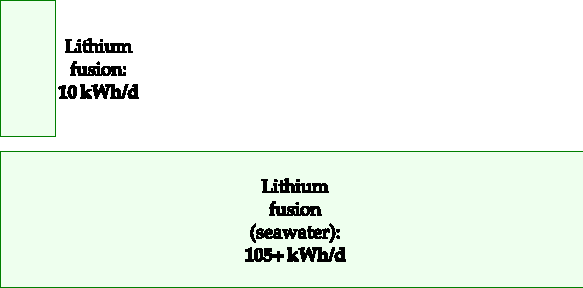
\includegraphics{fig/intro/lithium}
        \caption{
        Sustainability of the D-T fusion process.
        Mined lithium could yield $10 \text{kWh/day/person}$ for $10^{3}$ years.
        Seawater lithium could yield $105 \text{kWh/day/person}$ for around $10^{6}$ years.
        Based on the calculations in \cite{ongena2012,Eckhartt1995}.
        Note: Different scale than \cref{fig:energyConsumption}.
        }

        \label{fig:lithium}
    \end{subfigure}
    \vfill
    \begin{subfigure}[h]{1.00\textwidth}
        \centering
        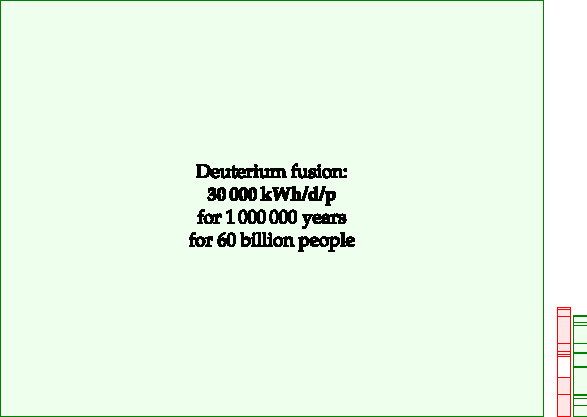
\includegraphics{fig/intro/DDFusion}
        \caption{
        Theoretical sustainability of the D-D process.
        The stacks from \cref{fig:energyConsumption} is shown for comparison.
        }
        \label{fig:DDFusion}
    \end{subfigure}
    \caption{Potential benefits and sustainability of fusion energy.
    Taken from \cite{Mackay2009book}}
    \label{fig:potFusion}
\end{figure}
%

\noindent
The problem of magnetical fusion can be boiled down to the following quote by Sebastien Balibar \cite{Balibar2009Web}:
%
\begin{quote}
    Fusion is like trying to put the Sun in a box - but we don't know how to make the box.
\end{quote}
%
Although a fairly good idea of what the "box" should look like has emerged the last decades, there are still challenges waiting to be solved.
The "box" which until now has proven most successful is the tokamak, depicted in \cref{fig:tokamak}
%
\begin{figure}[htb]
    \begin{center}
        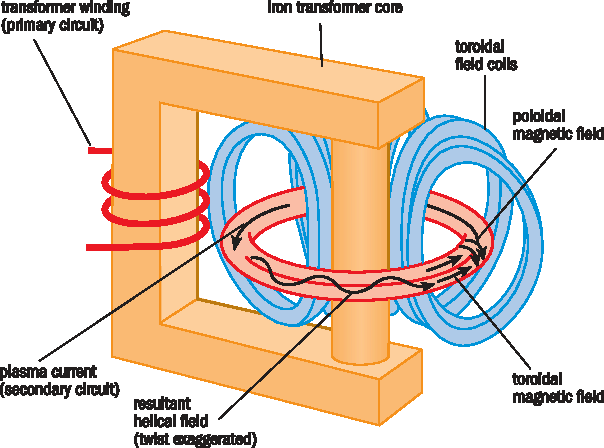
\includegraphics{fig/intro/tokamak}
    \end{center}
    \caption{Simplified schematics of the tokamak. From \cite{nuttall2008}}
    \label{fig:tokamak}
\end{figure}

\noindent



YOU ARE HERE
tokamaks



Problems with plasmas in the scrape-off layer
How is the energy distributed between the divertor tiles and the first wall


ITER achieve a high Q, the success will be lessened if the divertor tiles melt or the first wall is destroyed.



Therefore: A linear machine is good:
Easier to understand as there is no curvature drive
The simplemost system which is still encapturing the detail we are interested in

Easier to diagnose
Benchmarking of codes
Are they fusion relevant?
Material testing (not considered here)
Detachment studies (also not considered here)
Studies of non-curvature instabilities (actually considered here)
Can be similar to the SOL in fusion machines
Instabilities like drift-waves can be analgous to temperature
gradient modes found in fusion machines

If we would like to find the time a whit ball takes to fall.
Does it matter that the ball is white?
One could imagine that there are some reflection properties of the white ball which alters the fall-time.
However, such an effect would most likely be negligible.
The fact that the ball is white would be far more relevant if we would like to find the cooling time of the ball.
Thus, we have to ask the question: What kind of glasses are we using when investigating the physical phenomenon.

Hasegawa-Mima and Hasegawa-Wakatani only following fluctuations

Fluctuations can be big, so should finer model
CYTO is another model which takes this global approach when simulating a linear device.










Top down approach
Better predictability together with a better understanding of the underlying physical process.

As such, this thesis does not answer the ultimate question
how can the plasma be operated in order to make man made fusion energy be economically viable
daunting task.

Instead, questions related to the ultimate question is touched.
More presicely, this thesis tries to aswer the following questions.
Questions answered
To what extent does the Boussinesq approximation alters the solution of a model without the Boussinesq approximation.
(Does our model capture the features reported in the literature?)
Can coherent structures as blobs and holes be found from our model
Are zonal flows found in our model?
What numerical approaches can be used in order to model the scrape-off layer


\section{Thesis structure}
%
The remainder of this thesis is structured into $6$ main-parts.

As we would like to simulate a set of equation derived more or less from first priciples, the \cref{part:CELMA} is dedicated to the derivation of the CELMA model.
To enable full transparency of the derivation, most intermediate calculation step are also shown.
As such, this thesis is addressed to a readership familiar with basic concepts of plasma physics.
Readers familiar with these derivations may readily skip these intermediate steps, but should pay extra attention to the derivation of the modified vorticity equation, as (to the authors best knowledge) this is not given elsewhere.
In \cref{chap:kin} the derivation of the fluid equations is done by taking moments of the Fokker-Planck equation including a particle source.
The first two fluid moments is taken, and the fluid closure is done by assuming a constant temperature.
These equations are further refined using the drift-fluid approximation in \cref{chap:drift-order}, where also the fluid drifts are given.
In \cref{chap:slowB} we restrict the system to only be valid for a slowly varying $B$-field, whereas in chapter \cref{chap:CELMA} a straigth magnetic field in a cylinder geometry is imposed.
The boundary conditions of the model is also given in \cref{chap:CELMA}.
The alternative model, which uses the Boussinesq approximation is given in chapter \cref{chap:boussinesq} before \cref{part:CELMA} is concluded by a summary.

In \cref{part:impl} all the details of the numerical implementation is given.
\Cref{chap:implBOUT++} describes the built-in options from the BOUT++ framework which is used in this thesis, and is followed by implementations which are not included in the BOUT++ in \cref{chap:additionalImplementation}.
The verification of the numerical implementation is given in \cref{chap:verification}.

Finally, the results from the numerical simulations are given in \cref{part:results}.
The setup is briefly given in \cref{chap:setup}, followed by a description of the phases of the model in chronological order.
\Cref{chap:ss} describes the steady state found from the simulations.
The system is perturbed and the following linear state is described in \cref{chap:linear} together with simplified linear drift wave theory.
The resulting turbulent state is presented in \cref{chap:satTurb}, and the characteristic of the fluctuation is given in \cref{chap:charTurb}.
% FIXME
FIXME \cref{chap:zonal} not given.
Investigation of how the system scales with varying $B$-field strength is given in \cref{chap:BFScan}, and the comparison with the model using Boussinesq approximation is given in \cref{chap:compBouss}.
% FIXME
FIXME \cref{chap:neutScan} not given.

A summary of the conclusion and outlook of this thesis is given in \cref{part:concl}.

To supplement, appendices are given in \cref{part:app}. These appendices are being referred to throughout the text with exception of \label{app:shortcomings} which summarises the shortcomings in this thesis.
